% !TeX spellcheck = en_GB
\PassOptionsToPackage{square,comma,numbers,sort&compress}{natbib}

\documentclass{article}

\usepackage[preprint]{neurips_2019}

\usepackage[utf8]{inputenc} % allow utf-8 input
\usepackage[T1]{fontenc}      % use 8-bit T1 fonts
\usepackage{hyperref}      		 % hyperlinks
\usepackage{url}            			% simple URL typesetting
\usepackage{booktabs}     		 % professional-quality tables
\usepackage{tabularx}
\usepackage{multirow}
\usepackage{nicefrac}      		  % compact symbols for 1/2, etc.
\usepackage{microtype}     		% microtypography
\usepackage[inline]{enumitem}
\usepackage{amsmath}
\usepackage{amsfonts}       	 % blackboard math symbols
\usepackage{bm}
\usepackage{mathtools} 
\usepackage {xcolor}
%\usepackage[section]{placeins} % Prevent figures from being moved across sections
% Reset subcaption counters at the start of figure/table float
\usepackage{subcaption}

\title{ATML Report}

\author{%
		Giorgia Adorni \\
		\texttt{giorgia.adorni@usi.ch} \\
		\And
		Felix Boelter\\
		\texttt{felix.boelter@usi.ch}\\
		\And
		Stefano Carlo Lambertenghi\\
		\texttt{stefano.carlo.lambertenghi@usi.ch}\\
}

\begin{document}
	
	\maketitle
	\begin{abstract}
		%Train a GAN with Transformer-like architecture
		%Concise and self-contained description of your project, motivation and main findings.
		The field of image origination through generative modeling is abundantly discussed at
		the moment, as it can be used for an extremely varied range of applications such as 
		up-scaling already existing images, creating non-existing objects such as interior 
		design scenes, products or even human faces but also to achieve transfer-learning 
		processes.
		In this context, GANs (Generative Adversarial Networks) are a class of widely studied 
		machine learning frameworks first appeared in the paper 
		``\emph{Generative adversarial Nets}'' by \citet{goodfellow2014generative} that achieve
		the aforementioned goal.
		In our work we will reproduce and evaluate a novel variation of the original GAN 
		network, the GANformer, proposed in  ``\emph{Generative adversarial Transformers}'' by 
		\citet{hudson2021generative}.
	\end{abstract}

	%	\section*{General notes}
	%	
	%	The report should be written as an article intended to present the findings of your work. Your 
	%	aim should be to be clear and objective, substantiating your claims with references or 
	%	empirical/theoretical evidence.
	%	
	%	We are well aware of the fact that carrying out machine learning experiments might be difficult 
	%	and that often the final performance might be disappointing. For this reason, you will not be 
	%	evaluated solely on quantitative aspect of your work, but mainly on the quality of your analysis 
	%	and report.
	%	
	%	The length of the report should be between 4 and 8 pages (without considering references).
	
	\section{Introduction}
	This objective of this project is to investigate the reliability and reproducibility of a paper accepted 
	for publication in a top machine learning conference.
	The models have been implemented using code and information provided by the authors.	
	Actually we are not participating formally to the \textit{Fall Edition of the ML Reproducibility 
	Challenge 2021}.
	
	With this work, we are going to verify the empirical results and claims of the paper 
	``\emph{Generative adversarial transformers}'' by \citet{hudson2021generative}, by reproducing 
	three of the computational experiments performed by the authors:
	\begin{enumerate*}
		\item[(1)] the \textbf{StyleGAN2} by \citet{karras2020analyzing,karras2019style}, a GAN 
		network which uses one 
		global latent style vector to modulate the features of each layer, hence to control the style of all 
		image features globally,
		\item[(2)] the \textbf{GANformer} with \textbf{Simplex Attention} by 
		\citet{hudson2021generative}, a generalisation of the StyleGAN design with \textit{k} latent 
		vectors that cooperate through attention, allowing for a spatially finer control over the generation 
		process since multiple style vectors impact different regions in the image concurrently, in 
		particular permitting communication in one direction, in the generative context – from the latents 
		to the image features, and
		\item[(3)] the \textbf{GANformer} with \textbf{Duplex Attention} by \citet{hudson2021generative}, 
		which is based on the same principles as the previous but propagating information both from 
		global latents to local image features, enabling both top-down and bottom-up reasoning to occur 
		simultaneously.
	\end{enumerate*} 
	
	The first model is used as baseline, while the remaining are the architectures introduced by the 
	authors. Thy consider the GANformer has ``a novel and efficient type of transformer'' which 
	demonstrates its strength and robustness over a range of task of visual generative modelling —  
	simulated multi-object environments (real-world indoor and out-door scenes) — achieving 
	state-of-the-art results in terms of both image quality and diversity, while benefiting from fast 
	learning and better data-efficiency. 
	
	% TODO ummary of the main results and contributions

	\section{Related works/Background}	
	
	\subsection{Generative Adversarial Networks (GANs)}\label{sec:gan}
	Generative Adversarial Networks (GANs) \cite{goodfellow2014generative}, are deep-learning-based 
	generative models which learn to determine whether a sample is from the model or the data 
	distribution. 
	
	The classic architecture is composed by two main neural networks: the \textit{generator} ${G(z)}$, 
	which take as input a sample from the latent space $z$, or a vector drawn randomly from a 
	Gaussian distribution, and use it to generate new plausible examples in the problem domain — 
	images in our case — , and the \textit{discriminator} ${D(x)}$, which takes an example from the 
	domain as input, and predicts a binary class label which classify the examples as real (coming from 
	the training dataset) or fake (generated by $G$).
	
	The two models are trained together: the discriminator $D$ estimates the probability that 
	sample $x$ is generated by $G$ or is a real sample, and aims at maximising the probability of 
	assigning the correct label to both real and fake samples, while the generator $G$ is trained to 
	maximise the probability of the discriminator $D$ making a mistake, so it aims to minimise 
	$\log(1-D(G(z))))$.

	Combining the two objectives for $G(z)$ and $D(x)$ we get the \textit{GAN min-max game} with the 
	value function $V(G,D)$:
	\begin{equation}
	\label{e:minmaxgame}
	\min_G \max_D V(G,D) = 
	\mathbb{E}_{x \sim p*(x)} [\log D(x)] + \mathbb E _{z \sim p_z(z)} [\log (1-D(G(z))))]
	\end{equation}
	
	GANs typically work with images, as in our case, for this reason, both the generator and 
	discriminator models use Convolutional Neural Networks (CNNs).
	
	\subsection{StyleGAN2}\label{sec:stylegan}%TODO fixme
	StyleGAN are a re-design of the GANs generator architecture, which aim is to control the image 
	synthesis process \cite{karras2019style}.
	
	The StyleGAN approach departs from the design of a common generator network, consisting in a 
	multi-layer CNN.
	A traditional GAN generator feeds the latent code $z$ though the input layer only, to start the 
	up-sampling process.
	\citet{karras2019style} introduce a feed-forward mapping network $f : Z \rightarrow W$ which 
	processes the latent code $z$ in the input latent space $Z$, and output an intermediate latent 
	vector $w \in W$. 
	$w$, in turn, interacts directly with each convolution through the synthesis network  $g$ and, in 
	particular, with the \textit{Adaptive Instance Normalisation (AdaIN)} \cite{huang2017arbitrary} aligns 
	the mean and variance of the content features with those of the style features, meaning that ia able 
	to globally controls these parameters and so the strength of image features at different scales. 
	
	The \textit{AdaIN} operation is defined as:
	\begin{equation}
		\label{e:adain}
		\mathsf{AdaIN}(x, y) = \sigma(y) \bigg(\frac{x - \mu(x)}{\sigma (x)} \bigg) + \mu (y) \mbox{,}
	\end{equation}
	where $x$ is the content input, $y$ a style input, and the channel-wise mean and variance of $x$ 
	are aligned to match those of $y$.

	Moreover, by introducing explicit Gaussian noise inputs after each convolution, 
	\citet{karras2019style} provide the generator with a direct means to generate stochastic detail: an 
	automatic and unsupervised separation of high-level attributes (e.g., pose, identity) from stochastic 
	variation (e.g., freckles, hair) is obtained in the generated images, and intuitive scale-specific mixing 
	and interpolation operations are enabled.
	
	StyleGAN2 \cite{karras2020analyzing} are a revisiting of the architecture of the StyleGAN. 
	In particular, some redundant operations have been removed from the original StyleGAN architecture.
	Bias and noise are operations which might have conflicting interests, and their application within the 
	style block caused their relative impact to be inversely proportional to the current style’s 
	magnitudes. For this reason, they have been moved outside the style block and separated, allowing 
	to obtain more predictable results.
	Furthermore, after this change, the mean is no longer necessary, but it is sufficient for the 
	normalisation and modulation to operate on the standard deviation alone.
	Moreover, the application of bias, noise, and normalization to the constant input has been safely 
	removed. 
	
	%TODO from here on the text does not convince me
	\textcolor{red}{
	When the style block consists in a modulation, a convolution, and a normalisation operation, it is 
	possible to restructure the AdaIN has a demodulation operation, which is applied to the weights 
	associated with each convolution layer. 
	AdaIN uses different scale and shift parameters to align different areas of $w$ — the activations of 
	intermediate activations — with different regions of the feature map (either within each feature map 
	or via grouping features channel-wise by spatial location), while weight demodulation takes the scale 
	and shift parameters out of a sequential computation path, instead baking scaling into the 
	parameters of convolutional layers.}
	
	\textcolor{red}{
	The StyleGAN2 architecture makes it possible to control the image synthesis via scale-specific 
	modifications to the styles. In particular, this approach attains layer-wise decomposition of visual 
	properties, allowing StyleGAN to control global aspects of the picture such as pose, lighting 
	conditions or colour schemes, in a coherent manner over the entire image.}
	
	\textcolor{red}{
	But while StyleGAN successfully disentangles global properties, it is more limited in its ability to 
	perform spatial decomposition, as it provides no direct means to control the style of a localized 
	regions within the generated image.}

	\subsection{Transformers}%TODO fixme
	Transformers are deep learning models based on an \textit{attention mechanism} designed to handle 
	sequential input data and evaluate the relationship between each input-output item 
	\cite{vaswani2017attention}.
	This models, unlike Recurrent Neural Networks (RNNs), avoid using convolutions or aligned 
	sequence, and do not necessarily require ordered input data to be processed. 
	
	The architecture is composed by an encoder-decoder structure where, the \textit{encoder} maps an 
	input sequence of symbol representations $(x_1,\dots, x_n)$ to a sequence of continuous 
	representations $z = (z_1, \dots, z_n)$, while the  \textit{decoder}, given $z$, generates an 
	output sequence $(y_1, \dots, y_m)$ of symbols one element at a time. 
	Each transformer module (encoder-decoder) is connected to each other via feed-forward layers.
	
%	At each step the model is auto-regressive, consuming the previously generated symbols as 
%	additional input when generating the next.
%		\begin{enumerate*}
%			\item[(1)] a \textit{multi-head self-attention mechanism} working in parallel, and 
%			\item[(2)] a \textit{position-wise fully connected feed-forward neural network}, with residual 
%			connections followed by normalisation.
%	\end{enumerate*}
%	Moreover, the decoder self-attention sub-layer has a mask which prevents positions from 
%attending 
%	to subsequent positions (so positional encoding provided as additional input to bottom layer). 
%This, 
%	combined with fact that the output embeddings are offset by one position, ensures that the 
%	predictions for position $i$ can depend only on the known outputs at positions less than $i$.
% 	In addition, the decoder has a third sub-layer, which performs \textit{multi-head attention} over the 
% 	output of the encoder stack. 
	
	An \textit{attention function} \cite{vaswani2017attention}, can be described as mapping a query and 
	a set of key-value pairs to an output, where the query, keys, values, and output are all vectors. The 
	output is computed as a weighted sum of the values, where the weight assigned to each value is 
	computed by a compatibility function of the query with the corresponding key.

	The input consists of queries and keys of dimension $d_k$, and values of dimension $d_v$. The dot 
	products of the query with all keys is computed, each divided by $\sqrt{d_k}$ and then a 
	softmax function is applied to obtain the weights on the values.
	In practice, the attention function is computed on a set of queries simultaneously, packed together 
	into a matrix $Q$. The keys and values are also packed together into matrices $K$ and $V$. 
	\begin{equation}
		\label{eqn:attention}
		\mathsf{Attention}(Q, K, V) = \mathsf{softmax} \big( \frac{QK^T}{\sqrt{d_k}}\big)V
	\end{equation}
	% This is a \textit{dot-product attention} with a scaling factor of $\sqrt{1}$. 
			
	Instead of performing a single attention function, transformers use multiple self-attentions, called 
	\textit{multi-head attention}, allowing the model to jointly attend to information from different 
	representation subspaces at different positions, learning attention relationship independently	
	\cite{vaswani2017attention}.
	\citet{vaswani2017attention} used multiple multi-head attentions stacked on the top of each other, 
	in this way, the parallel attention layers enables to pass multiple input sequences simultaneously 
	instead of one at a time, allowing for more parallelisation and therefore reducing training times if you 
	have access to sufficient computational resources.
	
	\begin{equation}
		\label{eqn:multihead}
		{\mathsf{MultiHead}(Q, K, V) = \mathsf{Concat}(\mathsf{head}_1 \dots, 
		\mathsf{head}_h) W^O }
		\mbox{,}
	\end{equation}
	where $ \mathsf{head}_i = \mathsf{Attention}(QW_i^Q, KW_i^K , VW_i^V)$, and the 
	projections are parameter matrices $W_i^Q \in \mathbb{R}^{d_{\text{model}}\times 
	d_k}$, %TODO $W_i^Q \in \mathbb{R}^{d_{\text{model}}\times d_q}$,  probabile errore
	$W_i^K \in \mathbb{R}^{d_{\text{model}}\times d_k}$, $W_i^V \in 
	\mathbb{R}^{d_{\text{model}}\times d_v}$ and $W^O \in \mathbb{R}^{hd_v \times 
	d_{\text{model}}}$.
	
	%TODO repetition: integrate in the previous text
	\textcolor{blue}{
	The transformer uses multi-head attention in three different ways:
	\begin{enumerate}
		\item In "encoder-decoder attention" layers, the queries come from the previous decoder layer, 
		and the memory keys and values come from the output of the encoder. This allows every position 
		in the decoder to attend over all positions in the input sequence.
		\item The encoder contains self-attention layers, in which all of the keys, values 
		and queries come from the output of the previous layer in the encoder. 
		Each position in the encoder can attend to all positions in the previous layer of the encoder.
		\item Similarly, self-attention layers in the decoder allow each position in the decoder to attend to 
		all positions in the decoder up to and including that position. We need to prevent leftward 
		information flow in the decoder to preserve the auto-regressive property. We implement this 
		inside of scaled dot-product attention by masking out (setting to $-\infty$) all values in the input 
		of the softmax which correspond to illegal connections. 
	\end{enumerate}
	}
	
	\section{Methodology}
	%	In this section you should give a description of the methodological aspects of your work, for 
	%	instance how you modified an existing method to perform a particular task or to overcome a 
	%	particular limitation. If your project is about reproducibility, here you should describe the method 
	%	presented in the original paper.
	
	\subsection{Generative Adversarial Transformers}%TODO fixme	
	The Generative Adversarial Transformers (GANsformer), as presented in 
	\cite{hudson2021generative}, are models which combine GANs and the transformers to generate 
	better and more realistic examples.
	
	GANs are exploited in this architecture since they work with CNNs, and for this reason they are 
	powerful generators for the overall style of the image, since by nature they merge the local 
	information of the pixels together with the general information regarding the image. 
	However, they are less powerful regarding small details of localised regions within the generate 
	image itself, since they miss out on the long range interaction of the faraway pixel.
	
	Styegan2...
	
	Accordingly, GANsformer take advantage of the transformers attention mechanism to make the 
	StyleGAN2 architecture even more powerful: the integration of attention in the architecture allows 
	the network to draw global dependencies between input and output, and understand the context of 
	the image thanks to the transformer's strength for long-range interactions.
	Thus, rather than focusing on using global information and controlling all features globally, 
	transformer use attention to propagate information from the local pixels to the global high-level 
	representation and vice versa. 
	
	%TODO from here on the text does not convince me
	The \textit{bipartite transformer} structure computes \textit{soft attention}, iteratively aggregating 
	and disseminating information between the generated image features and a compact set of 
	\textit{latent variables} enable bidirectional interaction between these dual representations. 
	
	The \textit{transformer network} corresponds to the \textit{multi-layer bidirectional transformer 
	encoder} (BERT) described by \citet{devlin2019bert}, which interleaves \textit{multi-head 
	self-attention} and \textit{feed-forward layers}.
	Each pair of self-attention and feed-forward layers is intended as a \textit{transformer layer}, hence, 
	a transformer is a stack of several such layers. 
	
	The \textit{self-attention layer} considers all pairwise relations among the input elements, so to 
	update each single element by attending to all the others. 
	The \textit{bipartite transformer} generalises this formulation, featuring instead a bipartite graph 
	between two groups of variables — in the GAN case, latents and image features. 
	There are two attention operations that could be computed over the bipartite graph, depending on 
	the direction in which information propagates, 
	\begin{enumerate*}
		\item [(1)] \textit{simplex attention} permits communication either in one way only, in the 
		generative context, from the latents to the image features, and
		\item [(2)] \textit{duplex attention} which enables it both top-down and bottom-up ways.
	\end{enumerate*}
	
	Attention can be used in several ways: 
	\begin{enumerate}
		\item Simplex Attention: when attention is applied in one direction only from the latents to the 
		image features (top-down).
		\item Duplex Attention: when attention is applied in the two directions: latents to image features 
		(top-down) and then image features back to latents (bottom-up), so that each representation 
		informs the other iteratively.
		\item Self Attention between latents: can also be used so to each direct interactions between the 
		latents.
		\item Self Attention between image features (SAGAN model): prior approaches used attention 
		directly 
		between the image features, but this method does not scale well due to the quadratic number of 
		features which becomes very high for high-resolutions.
	\end{enumerate}

	In particular, the attention layers are added in between the convolutional layers of both the 
	generator and discriminator.
	
	The discriminator model performs multiple layers of convolution downsampling on the image, 
	reducing the representation's resolution gradually until making final prediction. 
	Optionally, attention can be incorporated into the discriminator as well where it has multiple $k$ 
	aggregator variables, that use attention to adaptively collect information from the image while being 
	processed. We observe small improvements in model performance when attention is used in the 
	discriminator, although note that most of the gain in using attention based on our observations 
	arises from the generator.
	%TODO until here
	
	
	\subsubsection{Simplex attention}%TODO fixme: reduce
	As already mentioned, simplex attention distributes information in a single direction over the 
	bipartite transformer graph. 
	
	Formally, let $X^{n\times d}$ denote an input set of $n$ vectors of dimension $d$ — where, for the 
	image case, $n = W\times H$ — and $Y^{m\times d}$ denote a set of $m$ aggregator variables — 
	the latents, in the generative case. Specifically, the attention is computed over the derived bipartite 
	graph between these two groups of elements, as in Equation \eqref{eqn:attention}, moreover:
	\begin{equation}
		\label{eqn:attention2}
		a(X,Y)=\mathsf{Attention}(q(X), k(Y), v(Y)) \mbox{,}
	\end{equation}
	where $q(\cdot), k(\cdot), v(\cdot)$ are functions that respectively map elements into queries, 
	keys, and values, all maintaining dimensionality $d$. 
	The mappings are provided with positional encodings to reflect the distinct position of each element 
	(e.g. in the image). This bipartite attention is a generalisation of self-attention, where $Y = X$.
	
	Standard transformers implement an additive update rule of the form:
	\begin{equation}
		\label{eqn:layernorm}
		u^a(X, Y)=\mathsf{LayerNorm}(X + a(X, Y)) \mbox{,}
	\end{equation}
	however, \cite{hudson2021generative} used the retrieved information to control both the scale as 
	well as the bias of the elements in $X$, in line with the practice promoted by the StyleGAN model 
	\cite{karras2019style}:
	\begin{equation}
		\label{eqn:simplex}
		u^s(X, Y)=\gamma (a(X, Y)) \odot \omega (X) + \beta (a(X, Y)) \mbox{,}
	\end{equation}
	where $\gamma(\cdot), \beta(\cdot)$ are mappings that compute multiplicative and additive styles 
	(gain and bias), maintaining dimensionality $d$, and $\omega (X) = X- \mu(X)$ normalises each 
	element with $\sigma(X)$ respect to the other features. By normalizing $X$ (image features), and 
	then letting $Y$ (latents) control the statistical tendencies of $X$, the information propagation from 
	$Y$ to $X$ is enabled, allowing the latents to control the visual generation of spatial attended 
	regions within the image, so as to guide the synthesis of objects or entities.
	The multiplicative integration permits significant gains in the model performance. 
	
	\subsubsection{Duplex attention}%TODO fixme: reduce
	Duplex attention can be explained by taking into account the variables $Y$ to set their own 
	key-value structure: $Y = (K^{n\times d} , V^{n\times d})$, where the values store the content of the 
	$Y$ variables, as before (e.g. the randomly sampled latent vectors in the case of GANs) while the 
	keys track the centroids $K$ of the attention-based assignments between $Y$ and $X$, which can 
	be computed as $K = a(Y, X)$ — namely, the weighted averages of the $X$ elements using the 
	bipartite attention distribution derived through comparing it to $Y$. 
	Consequently, the new update rule is defined as follows:
	\begin{equation}
		\label{eqn:duplex}
		u^d(X, Y )=\gamma (A(X, K, V)) \odot \omega (X) + \beta (A(X, K, V)) \mbox{,}
	\end{equation}
	where, two attention operations are compound on top of each other: first compute the \textit{soft 
	attention} assignments between $X$ and $Y$, by $K = a(Y, X)$, and then refine the assignments by 
	considering their centroids, by $A(X, K, V)$. This is analogous to the \textit{k-means algorithm} and 
	works more effectively than the simpler update $u^a$ defined above in Equation \eqref{eqn:simplex}.
	
	Finally, to support bidirectional interaction between $X$ and $Y$ (the image and the latents), two 
	reciprocal simplex attentions are chain from $X$ to $Y$ and from $Y$ to $X$, obtaining the duplex 
	attention, which alternates computing $Y :=u^a(Y,X)$ and $X:=u^d(X,Y)$, such that each 
	representation is refined in light of its interaction with the other, integrating together bottom-up and 
	top-down interactions.
	
	\subsubsection{Vision-specific adaptations}%TODO fixme
	Some adaptations, that will be later described in Section \ref{sec:hyperparam}, have been applied to 
	the structure of the GANformer in order to foster an interesting communication flow. Rather than 
	densely modelling interactions among all the pairs of pixels in the images, instead it supports 
	\textit{adaptive long-range interaction} between far away pixels in a moderated manner, passing 
	through a compact and global latent bottleneck that selectively gathers information from the entire 
	input and distributes it back to the relevant regions. 
	
	\subsubsection{The Generator and Discriminator Networks}
	The StyleGAN2 model \cite{karras2019style, karras2020analyzing}, presented in Section 
	\ref{sec:stylegan}, is used as a starting point for the GAN design. 
		

	The generator likewise is composed of two parts:
	\begin{enumerate}
		\item The \textit{mapping network}, which consists in a series of feed-forward layers, whose 
		objective is to convert the sampled latents from a normal distribution $z$ to the intermediate 
		space $w$. The $k$ latent components either are mapped independently or interact with each 
		other through self-attention.
		\item The \textit{synthesis network} is composed by multiple layers of convolution where the 
		images features begin from a small constant/sampled grid and up-sampling until reaching the 
		desirable resolution.
		After each convolution, the image features are modulated by the intermediate latent vectors $w$, 
		meaning that their variance and bias are controlled. 
		While in StyleGAN2 a single global $w$ vector controls all the features equally, the GANformer 
		uses attention so that the $k$ latent components specialise to control different regions in the 
		image to create it cooperatively, and therefore perform better especially in generating images 
		depicting multi-object scenes, allowing also for a flexible and dynamic style modulation at the 
		region level.
	\end{enumerate}

	The bipartite transformer offers a solution to the StyleGAN limitation in its ability to perform spatial 
	decomposition which leaded to the impossibility of controlling the style of a localised regions within 
	the generated image.
	
	Instead of controlling the style of all features globally, the new attention layer is used to perform 
	\textit{adaptive region-wise modulation}. The latent vector $z$ is split into $k$ components, $z = 
	[z_1 , \dots, z_k ]$ and, as in StyleGAN \cite{karras2019style}, pass each of them through a shared 
	mapping network, obtaining a corresponding set of intermediate latent variables $Y = [y_1 , ..., y_k 
	]$. 
	
	During synthesis, after each CNN layer in the generator, the feature map $X$ and latents $Y$ play 
	the roles of the two element groups, mediating their interaction through our new attention layer 
	(either simplex or duplex). 
	This setting thus allows for a flexible and dynamic style modulation at the region level. 
	
	Since soft attention tends to group elements based on their proximity and content similarity, the 
	transformer architecture naturally fits into the generative task and proves useful in the visual 
	domain, allowing the model to exercise finer control in modulating local semantic regions. This 
	capability turns to be especially useful in modelling highly-structured scenes.
	
	For the discriminator, attention is applied after every convolution using trained embeddings to 
	initialise the aggregator variables $Y$, which may intuitively represent background knowledge the 
	model learns about the task. At the last layer are concatenated these variables $Y$ to the final 
	feature map $X$ to make a prediction about the identity of the image source. 
	This structure empowers the discriminator with the capacity to likewise model long-range 
	dependencies, which can aid it in its assessment of the image fidelity, allowing to acquire a more 
	holistic understanding of the visual modality.
	\textcolor{blue}{
	\begin{itemize}
		\item Compositional Latent Space with multiple variables that coordinate through attention to 
		produce the image cooperatively, in a manner that matches the inherent compositionality of 
		natural scenes.
		\item Bipartite Structure that balances between expressiveness and efficiency, modelling 
		long-range dependencies while maintaining linear computational costs.
		\item Bidirectional Interaction between the latents and the visual features, which allows the 
		refinement and interpretation of each in light of the other.
		\item Multiplicative Integration rule to impact the features' visual style more flexibly, akin to 
		StyleGAN but in contrast to the transformer network.
	\end{itemize}
}
	
	\section{Implementation}
	%	This section should be structured as follows (from the Reproducibility challenge template):
	%	
	%	---
	%	
	%	Briefly describe what you did and which resources did you use. E.g. Did you use author's code, 
	%	did you re-implement parts of the pipeline, how much time did it take to produce the results, 
	%	what hardware you were using and how long it took to train/evaluate. 
	
	The code has been implemented using code and information provided by the authors.
	
	\subsection{Datasets}	
	The original paper \cite{hudson2021generative} explored the GANformer model on four datasets for 
	images and scenes: CLEVR \cite{johnson2017clevr}, LSUN-Bedrooms \cite{yu2015lsun}, Cityscapes 
	\cite{cordts2016cityscapes} and FFHQ \cite{karras2019style}. 
	
	Initially, we tried to use the Cityscapes dataset, since it is the smaller among the four: it contains 
	24998 images with 256x256 resolution. 
	However, the time to complete the training was to high on this dataset (TODO: how much?), even if 
	using computational resources like GPU.
	
	For this reason, we switch to another dataset, the Google Cartoon Set \cite{cartoonset}\footnote{	
	\url{https://google.github.io/cartoonset}}, containing 10k 2D cartoon avatar 
	images with 64x64 resolution, composed of 16 components that vary in 10 artwork attributes, 4 
	colour attributes, and 4 proportion attributes (see in Table \ref{tab:dataset}). 

	\begin{table}[htb]%TODO maybe remove
		\centering
		\caption{Attributes of the Cartoon Set \url{https://google.github.io/cartoonset/download}.}
		\label{tab:dataset}
		\small
		\begin{tabularx}{\textwidth}{ll|r|X}
			&& \textbf{\# Variants} & \textbf{Description}                              \\
			\toprule
			\multirow{10}*{\textbf{Artwork}} 	&	\texttt{chin\_length}           & 3           & Length of chin 
			(below 	mouth region)      \\
			&	\texttt{eye\_angle}             & 3           & Tilt of the eye inwards or outwards      \\
			&	\texttt{eye\_lashes}            & 2           & Whether or not eyelashes are visible     \\
			&	\texttt{eye\_lid}               & 2           & Appearance of the eyelids      	\\
			&	\texttt{eyebrow\_shape}        & 14          & Shape of eyebrows        \\
			&	\texttt{eyebrow\_weight}        & 2           & Line weight of eyebrows           \\
			&	\texttt{face\_shape}            & 7           & Overall shape of the face                \\
			&	\texttt{facial\_hair}           & 15          & Type of facial hair (type 14 is no hair) \\
			&	\texttt{glasses}                & 12          & Type of glasses (type 11 is no glasses)  \\
			&	\texttt{hair}                   & 111         & Type of head hair                        \\
			\midrule
			\multirow{4}*{\textbf{Colors}} &	\texttt{eye\_color}    & 5 & Color of the eye irises           \\
			&	\texttt{face\_color}            & 11          & Color of the face skin                   \\
			&	\texttt{glasses\_color}         & 7           & Color of the glasses, if present         \\
			&	\texttt{hair\_color}        & 10     & Color of the hair, facial hair, and eyebrows      \\
			\midrule
			\multirow{4}*{\textbf{Proportions}} &	\texttt{eye\_eyebrow\_distance} & 3           & Distance 
			between the eye and eyebrows    \\
			&	\texttt{eye\_slant}             & 3           & Similar to eye\_angle, but rotates the eye and does 
			not change artwork  \\
			&	\texttt{eyebrow\_thickness}     & 4           & Vertical scaling of the eyebrows         \\
			&	\texttt{eyebrow\_width}         & 3           & Horizontal scaling of the eyebrows            \\
			\bottomrule                         
		\end{tabularx}
	\end{table}
	

	\subsection{Hyper-parameters}\label{sec:hyperparam}%TODO fixme
	%	Describe how you set the hyperparameters and what was the source for their value (e.g. paper, 
	%	code or your guess). 
	
	Note that in the code provided by the author \cite{hudson2021generative}, the hyper-parameters are 
	not the same mentioned in the article. 
	
	%TODO Vision specific adaptations
	A \textit{kernel size} of $k = 3$ is used after each application of the attention, together with a 
	\textit{Leaky ReLU non-linearity} after each convolution and then upsample or downsample the 
	features $X$, as part of the generator or discriminator respectively, as in e.g. StyleGAN2 
	\cite{karras2020analyzing}. 
	To account for the features location within the image, we use a sinusoidal positional encoding along 
	the horizontal and vertical dimensions for the visual features $X$, and trained positional 
	embeddings for the set of latent variables $Y$.
	Overall, the bipartite transformer is thus composed of a stack that alternates attention (simplex or 
	duplex), convolution, and upsampling layers, starting from a $4 \times 4$ grid up to the desirable 
	resolution. 
	
	Both the simplex and the duplex attention operations enjoy a bilinear efficiency of 
	$\mathcal{O}(mn)$ thanks to the network’s bipartite structure that considers all pairs of 
	corresponding elements from $X$ and $Y$. Since, as we see below, we maintain $Y$ to be of a fairly 
	small size, choosing m in the range of 8–32, this compares favourably to the prohibitive 	
	$\mathcal{O}(n^2)$  complexity of self-attention, which impedes its applicability to high-resolution 
	images.
	
	As to the loss function, optimization and training configurations, we adopt the settings and 
	techniques used in Style-GAN2 \cite{karras2020analyzing}, including in particular style mixing, 
	stochastic variation, exponential moving average for weights, and a non-saturating logistic loss with 
	a lazy R1 regularization.
	
	\subsection{Experimental setup}	
	The source code of our work is available at the following GitHub repository: 
	\url{https://github.com/GiorgiaAuroraAdorni/gansformer-reproducibility-challenge}.
	 
	 The approaches proposed in both the original paper codebase by \citet{karras2020analyzing} and 
	 by \citet{hudson2021generative} have been implemented in Python using TensorFlow 
	 \cite{tensorflow2015-whitepaper}, so, according to that, we used the same setup.
	 We created a Jupyter Notebook which runs all the experiments in Google Colaboratory, which 
	 allows us to write and execute Python in the browser. %TODO add google colab url
	
	 All the models have been trained on a Tesla P100-PCIE-16GB (GPU) provided by Google 
	 Colab Pro.
	
	\subsection{Computational requirements}%TODO fixme
	%	Provide information on computational requirements for each of your experiments. For example, 
	%   the  number of CPU/GPU hours and memory requirements. You'll need to think about this ahead 
	%	of time, and write your code in a way that captures this information so you can later add it to 
	%	this section. 
	In the original paper \cite{hudson2021generative}, they evaluate all models under comparable 
	conditions of training scheme, model size, and optimization details, implementing all the models 
	within the codebase introduced by the Style-GAN authors \cite{karras2020analyzing}. 
	All models have been trained with images of 256 × 256 resolution and for the 
	same number of training steps, roughly spanning a week on 2 NVIDIA V100 GPUs per model (or 
	equivalently 3-4 days using 4 GPUs). 
	
	Considered that we had available just one GPU and not enough time to reproduce this settings, we 
	decided to resize the images from 256×256 to 64x64 resolution.
	
	
	For the GANformer, we select k–the number of latent variables, from the range of 8–32. 
	
	All models have been trained for the same number of steps, which ranges between 5k to 15k kimg 
	training samples. 
	
	The paper present results after training 100k, 200k, 500k, 1m, 2m, 5m and 10m samples
	
	For the StyleGAN2 model we present results after training 100k (2h30m), 200k (6h), 500k, obtaining 
	good results.
	Note that the original StyleGAN2 model has been trained by its authors \cite{karras2020analyzing} 
	for up to 70k kimg samples, which is expected to take over 90 GPU-days for a single model. 
	

	For the GANformer, the authors \cite{karras2020analyzing} show impressive results, especially when 
	using duplex attention: the model manages to learn a lot faster than competing approaches, 
	generating astonishing images early in the training. This model is expected to take 4 GPU-days.
	
	However, we are not able to replicate this achievements, first because this model learns significantly 
	slower than the StyleGAN2, which is instead able to produce high-quality images in approximately 
	x-times less training steps than the GANformer.
	
	(in the paper they reach better results with the GANformer with 3-times less training steps than the 
	StyleGAN2, but they don't specify the time required for this training steps...)

	\section{Results}%TODO fixme
	%	In this section you should report the results of your work (e.g., the outcome of an empirical 
	%	analysis). You should be objective and support your statements with empirical evidence.
	%	
	%	Use figures, plots and tables to present your results in a nice and readable way.
	%	
	%	Refer to the Reproducibility Challenge template for hints on how to structure this in case you are 
	%	trying to replicate someone else's results.
	
	Sample images from different points in training are based on the same sampled latent vectors, 
	thereby showing how the image evolves during the training.
		
	For CLEVR and Cityscapes, we present results after training to generate 100k, 200k, 500k, 1m, and 
	2m samples. For the Bedroom case, we present results after 500k, 1m, 2m, 5m and 10m generated 
	samples during training
	
	These results show how the GANformer, especially when using duplex attention, manages to learn a 
	lot faster than competing approaches, generating impressive images early in the training
	
	\begin{figure*}[htpb]				
		\centering
		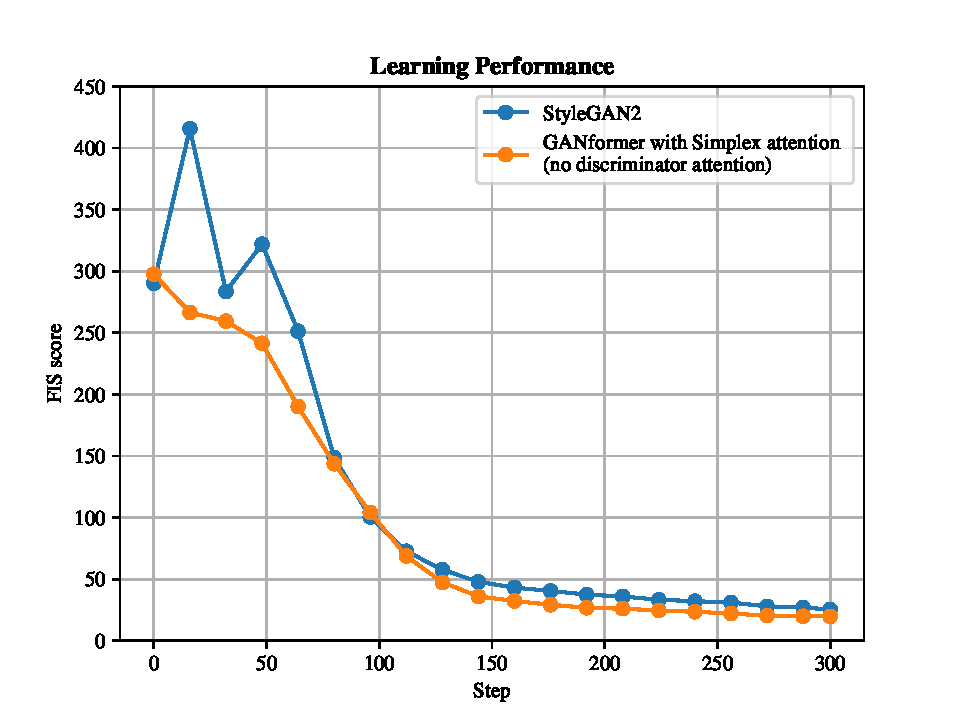
\includegraphics[width=.7\linewidth]{../src/trained_network/out_imgs/FIDscore.pdf}
		\caption{\textbf{Comparison between the StyleGAN2 and the GANformer models.} We evaluate 
		the models according to FID score along 300k image samples. The score is computed every 
		sixteen checkpoints.}
		\label{fig:performance}
	\end{figure*}
	
	The Frechet Inception Distance (FID) is one of the most popular metrics for evaluating GANs, which 
	provides stable and reliable indications of \textit{image fidelity} and \textit{diversity}. 
	It is a measure of similarity between curves that takes into account the location and ordering of the 
	points along the curves. 
	For this specific application, FID is used to measures the feature distance between the real and the 
	generated images, but it can be used for measuring the distance between two distributions as well.

	\begin{figure}[htpb]
		\centering
		\begin{subfigure}{\linewidth}
			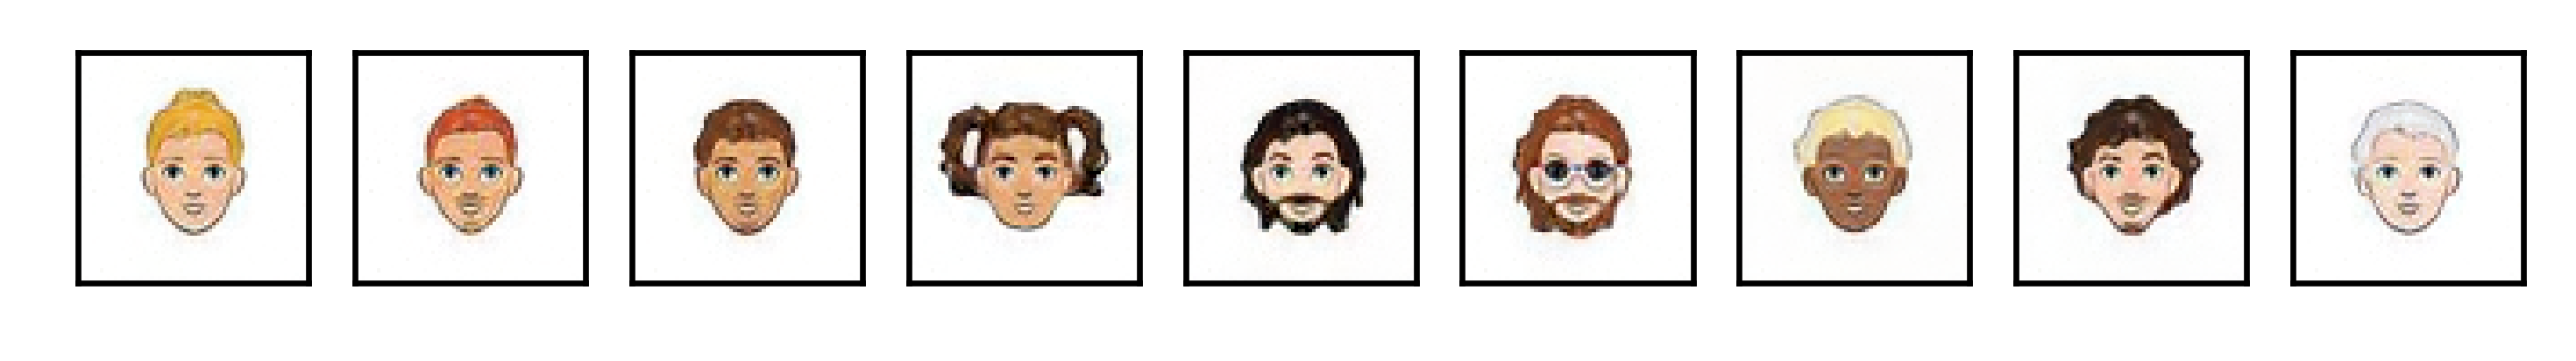
\includegraphics[width=\linewidth]{../src/trained_network/out_imgs/random_Stylegan2_300kimg.png}
			\vspace{-7mm}
			\caption{StyleGAN2.} 
		\end{subfigure}
		\begin{subfigure}{\linewidth}
			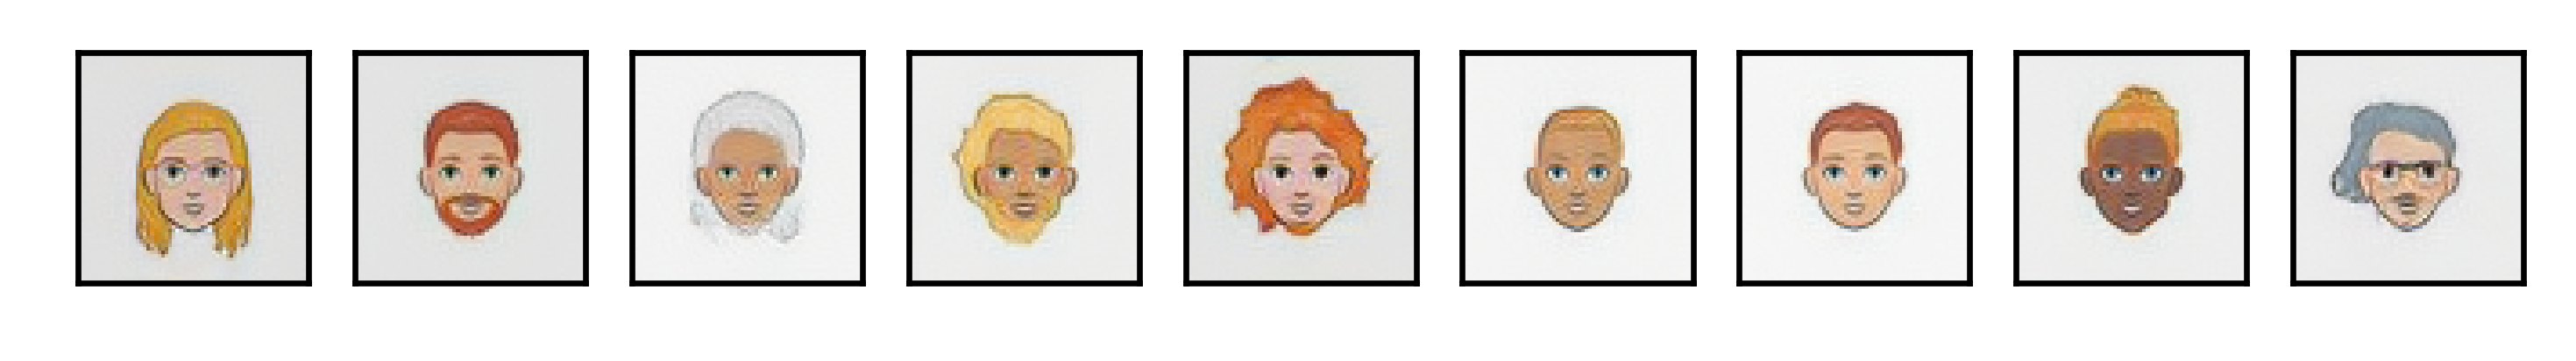
\includegraphics[width=\linewidth]{../src/trained_network/out_imgs/random_GANFormer_Simplex_D_StyleGAN_300kimg.png}
			\vspace{-7mm}
			\caption{GANformer model with Simplex attention and discriminator without attention.}
		\end{subfigure}
		\vspace{3mm}
		\caption{\textbf{Visualisation of 9 images generated with the various models}.}\label{fig:random}
	\end{figure}

	\begin{figure}[htpb]
		\centering
		\begin{subfigure}{\linewidth}
			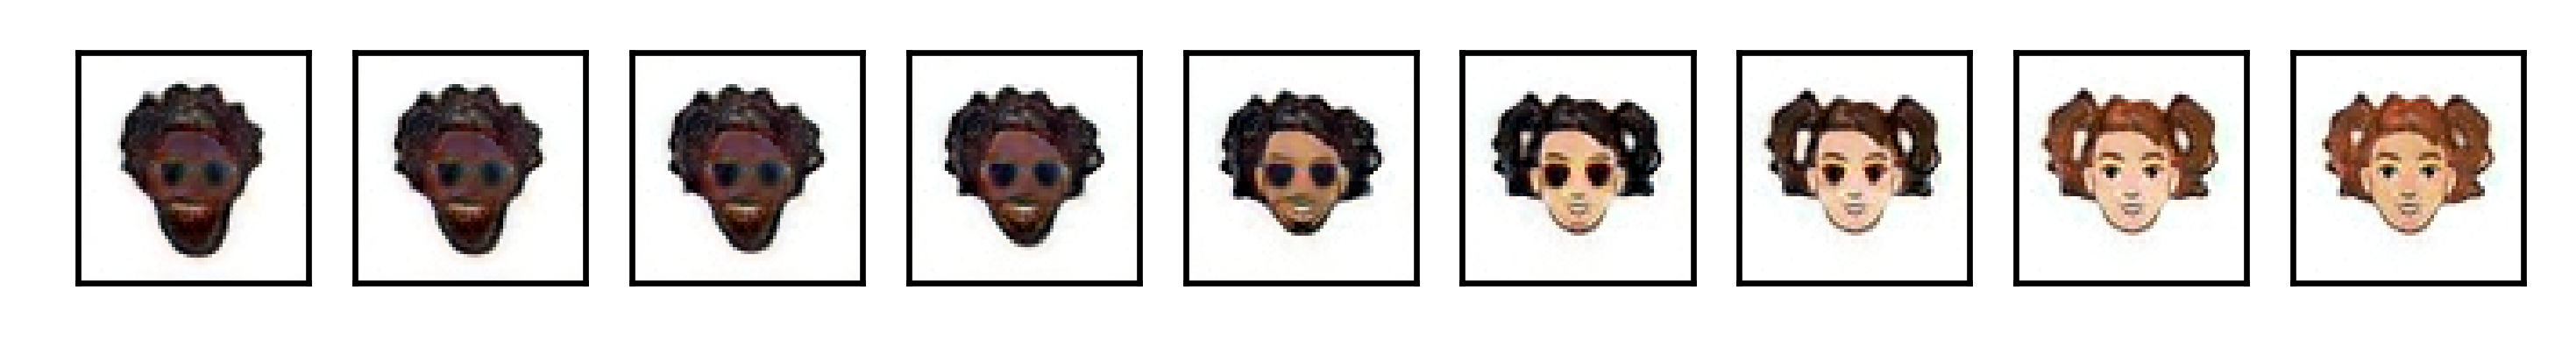
\includegraphics[width=\linewidth]{../src/trained_network/out_imgs/interpolation_Stylegan2_300kimg.png}
			\vspace{-7mm}
			\caption{StyleGAN2.} 
		\end{subfigure}
		\begin{subfigure}{\linewidth}
			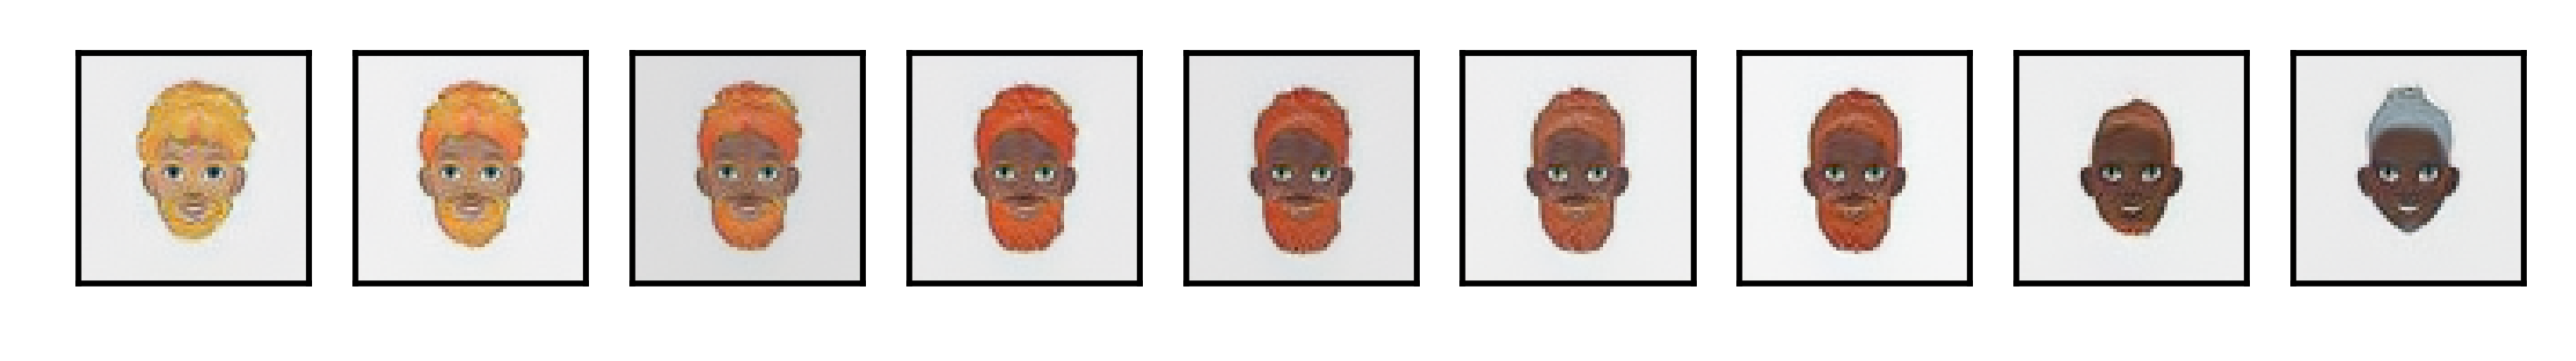
\includegraphics[width=\linewidth]{../src/trained_network/out_imgs/interpolation_GANFormer_Simplex_D_StyleGAN_300kimg.png}
			\vspace{-7mm}
			\caption{GANformer model with Simplex attention and discriminator without attention.}
		\end{subfigure}
		\vspace{3mm}
		\caption{\textbf{Simple $\mathbf{z}$ interpolation using of the various 
		models}.}\label{fig:interpolation}
	\end{figure}

	Visualisation of the models' comparison throughout the training. 

%	We evaluate the models along commonly used metrics such as FID, Inception Score IS, and 
%Precision \& Recall 
%	scores. 
	
%	We compute each metric 10 times over 50k samples, using different random seeds, and report their 
%	average.
	
%	The more layers attention is used through, the better the model’s performance gets and 
%	the faster it learns, confirming the effectiveness of the GANformer approach. 
	
	
	\section{Discussion and conclusion}%TODO
	%	Here you can express your judgments and draw your conclusions based on the  evidences 
	%	produced on the previous sections.
	%	
	%	Try to summarize the achievements of your project and its limits, suggesting (when appropriate) 
	%	possible extensions and future works.
	
	%TODO where should we put the author contributions?
	
	%%%web
	\clearpage %TODO remove this line at the end, its useful just to count the number of pages
	\bibliography{bibliography}
	\bibliographystyle{unsrtnat}
	\clearpage
	
\end{document}
